\documentclass[11pt,a4paper]{article}
\oddsidemargin 0.1 cm \evensidemargin 0.1cm \textwidth 16cm
\textheight24cm
\setlength{\topmargin}{0pt}\setlength{\headsep}{0pt}\pagestyle{empty}

\usepackage{graphicx}
\usepackage{variations}
\usepackage{enumerate}
\usepackage{amssymb}
\usepackage[latin1]{inputenc}  
\usepackage{fontenc}   
\usepackage{amsmath}
\usepackage{amsthm}
\usepackage{amsthm}
\usepackage{xypic}
\usepackage{variations}
%\usepackage{fancyhdr}
%\usepackage{xcolor}
%\usepackage{pstricks-add}
\usepackage[francais]{babel}
%\usepackage[french]{babel}
\newtheorem{defi}{D\'{e}finition}
\newtheorem{thm}{Th\'{e}or\`{e}me}
\newtheorem{rmq}{Remarque}
\newtheorem{prop}{Propri\'{e}t\'{e}}
\newtheorem{prop-def}{Propri\'{e}t\'{e}-D\'{e}finition}
\newtheorem{ex}{Exemple}
\newtheorem{exs}{Exemples}
\newtheorem{exer}{Exercice}
%\newtheorem{proof}{D\'{e}monstration}
\def\di{\displaystyle}
\newcommand{\vtab}{\rule[-0.4em]{0pt}{1.2em}}
\usepackage[top=0.5cm,bottom=0.5cm,right=1.5cm,left=1.5cm]{geometry}
\usepackage{pstricks,pst-plot} 
%\usepackage{framed}
\usepackage{amsmath}
%\usepackage{amssymb}
\usepackage{fancyhdr}
\usepackage{fancybox}
\usepackage{multicol}
%\usepackage{xcolor}
\usepackage{epsfig}
\usepackage{pifont}
%\usepackage[framed]{ntheorem}
%\usepackage[frenchb]{babel}
\usepackage{tabularx}
\def\R{{\mathbb R}}
\newtheorem{Rem}{Remarque}
\newcommand{\V}{\overrightarrow}
\newcommand{\Rep}{(O;\V{\imath};\V{\jmath})}
\newcommand{\Coor}[2]{\begin{pmatrix} #1\\#2 \end{pmatrix}}

\begin{document}
\title{}         % Enter your title between curly braces
\author{}        % Enter your name between curly braces
\date{}          % Enter your date or \today between curly braces
\maketitle
     
\indent\vspace{-3cm}

$$\fbox{\text{\Large{ Chapitre 1 - Feuille d'exercices n�2 : construction de la somme de deux vecteurs}}}$$
     
\hfill\\[0.2cm]

\noindent\underline{\textbf{Exercice 1 : }}\\
Dans chacun des cas suivants, construire le vecteur $\V{u}+\V{v}$ (sans sortir du quadrillage).\\
\psset{unit=0.5}
\begin{minipage}{0.3\linewidth}
$$\begin{pspicture}(10,10)
      \psgrid[gridlabels=0,subgriddiv=0,griddots=10](10,10)      
      \rput(2.5,7.5){$\V{u}$}
      \rput(4.5,2.5){$\V{v}$}
      \psline[linewidth=0.05cm]{->}(1,3)(4,9)
			\psline[linewidth=0.05cm]{->}(3,2)(7,1)
   \end{pspicture}$$
	\end{minipage}
	\begin{minipage}{0.3\linewidth}
$$\begin{pspicture}(10,10)
      \psgrid[gridlabels=0,subgriddiv=0,griddots=10](10,10)      
      \rput(3.4,8.7){$\V{u}$}
      \rput(1.5,2.5){$\V{v}$}
      \psline[linewidth=0.05cm]{->}(1,1)(4,3)
			\psline[linewidth=0.05cm]{->}(2,6)(5,10)
   \end{pspicture}$$
	\end{minipage}
	\begin{minipage}{0.3\linewidth}
$$\begin{pspicture}(10,10)
      \psgrid[gridlabels=0,subgriddiv=0,griddots=10](10,10)      
      \rput(3.5,4.5){$\V{u}$}
      \rput(7.5,1.5){$\V{v}$}
      \psline[linewidth=0.05cm]{->}(2,1)(6,7)
			\psline[linewidth=0.05cm]{->}(5,0)(10,2)
   \end{pspicture}$$
	\end{minipage}
\hfill\\
\\
\\


\noindent\underline{\textbf{Exercice 2 : }}\\
Dans chacun des cas suivants, construire les points $M$ et $N$ d�finis par les �galit�s vectorielles donn�es :\\
\\
\begin{minipage}{0.33\linewidth}
$$\V{OM}=\V{OA}+\V{OB}$$
$$\V{ON}=\V{BA}+\V{BC}$$
\hfill\\
\psset{unit=0.9}
$$\begin{pspicture}(12,7)
\psgrid[gridlabels=0,subgriddiv=0,griddots=10](12,7)   
\psdots(4,3)
\psdots(2,6)
\psdots(6,4)
\psdots(5,6)
\rput(3.5,2.5){$O$}
\rput(6.5,4.5){$A$}
\rput(4.5,6.5){$B$}
\rput(1.5,6.5){$C$}
\end{pspicture}$$
\end{minipage}
\begin{minipage}{0.33\linewidth}
$$\V{AM}=\V{OA}+\V{CB}$$
$$\V{AN}=\V{IJ}+\V{CJ}$$
\hfill\\
\psset{unit=0.9}
$$\begin{pspicture}(12,7)
\psgrid[gridlabels=0,subgriddiv=0,griddots=10](12,7)   
\psdots(2,6)
\psdots(5,6)
\psdots(4,3)
\psdots(4,4)
\psdots(5,3)
\psdots(6,4)
\rput(3.5,2.5){$O$}
\rput(4.5,2.5){$I$}
\rput(3.5,4.5){$J$}
\rput(6.5,4.5){$A$}
\rput(4.5,6.5){$B$}
\rput(1.5,6.5){$C$}
\end{pspicture}$$
\end{minipage}
\begin{minipage}{0.33\linewidth}
$$\V{EM}=\V{OA}+\V{OB}+\V{OC}$$
$$\V{AN}=\V{AB}+\V{AI}+\V{DI}$$
\hfill\\
\psset{unit=0.9}
$$\begin{pspicture}(12,7)
\psgrid[gridlabels=0,subgriddiv=0,griddots=10](12,7)   
\psdots(4,3)
\psdots(2,6)
\psdots(6,4)
\psdots(5,3)
\psdots(5,6)
\psdots(8,1)
\psdots(9,0)
\rput(3.5,2.5){$O$}
\rput(6.5,4.5){$A$}
\rput(4.5,6.5){$B$}
\rput(1.5,6.5){$C$}
\rput(4.5,2.5){$I$}
\rput(8.5,1.5){$D$}
\rput(9.5,0.5){$E$}
\end{pspicture}$$
\end{minipage}
\hfill\\


\noindent\underline{\textbf{Exercice 3 : }}\\
Construire � l'aide du compas, dans chacun des cas suivants, le vecteur $\V{u}+\V{v}$.\\
\\
\begin{minipage}{0.4\linewidth}
$$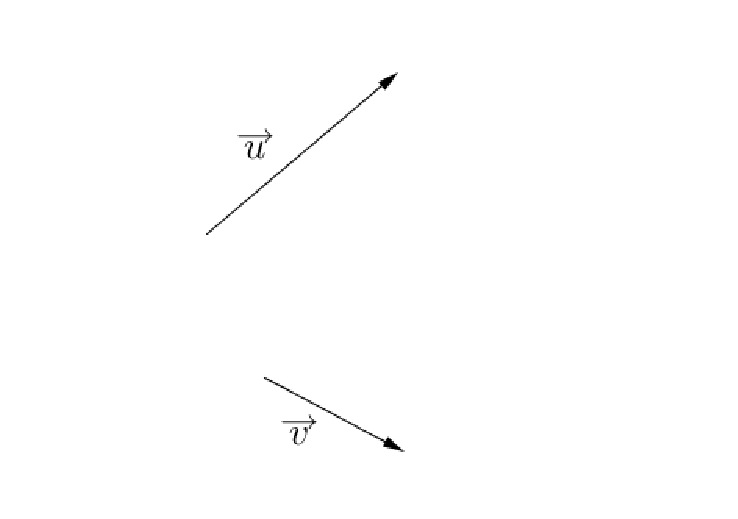
\includegraphics[scale=0.6]{exo-3-1.eps}$$
\end{minipage}
\begin{minipage}{0.6\linewidth}
$$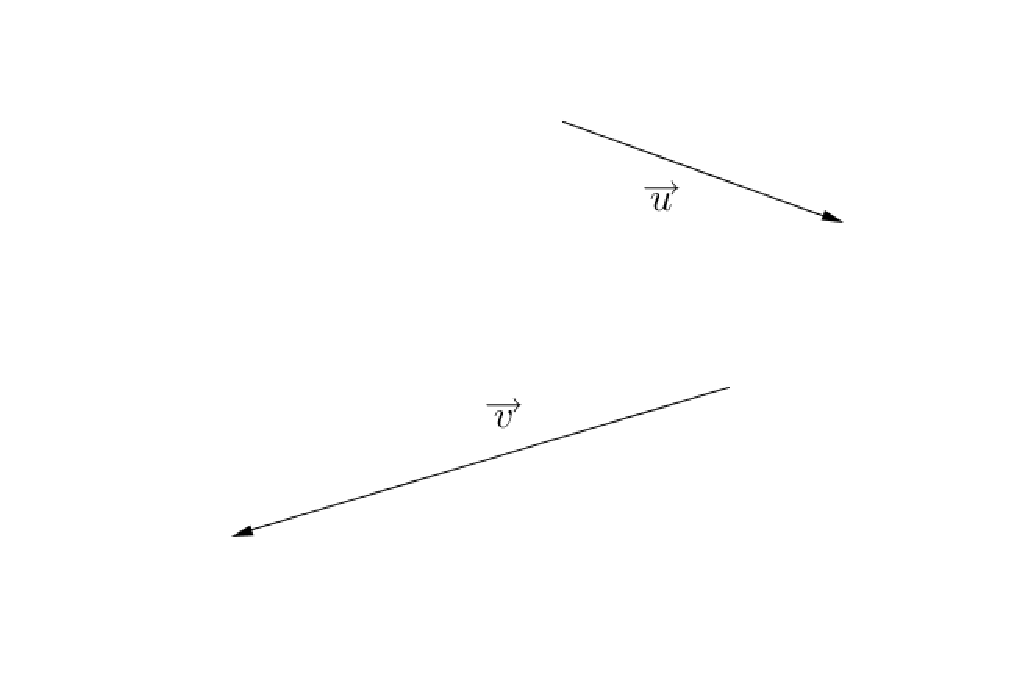
\includegraphics[scale=0.6]{exo-3-2.eps}$$
\end{minipage}
\hfill\\

\newpage

\noindent\underline{\textbf{Exercice 4 : }}\\  % Odyss�e 2014 p.180 exo 132
On consid�re les vecteurs repr�sent�s dans le quadrillage ci-dessous :

\psset{unit=1.8}
$$\begin{pspicture}(4,4)
\psgrid[gridlabels=0,subgriddiv=0,griddots=10](4,4)   
\psline{->,linewidth=0.055}(2,2)(2,3)
\psline{->,linewidth=0.055}(2,2) (3,3)
\psline{->,linewidth=0.055}(2,2) (3,2)
\psline{->,linewidth=0.055}(2,2) (3,1)
\psline{->,linewidth=0.055}(2,2) (2,1)
\psline{->,linewidth=0.055}(2,2) (1,1)
\psline{->,linewidth=0.055}(2,2) (1,2)
\psline{->,linewidth=0.055}(2,2) (1,3)
\rput(2,3.2){$N$}
\rput(3.2,3.2){$U$}
\rput(3.2,2){$E$}
\rput(3.2,0.8){$V$}
\rput(2,0.8){$S$}
\rput(0.8,0.8){$T$}
\rput(0.8,2){$O$}
\rput(0.8,3.2){$R$}
\rput(2.2,2.2){$P$}
\end{pspicture}$$


%$$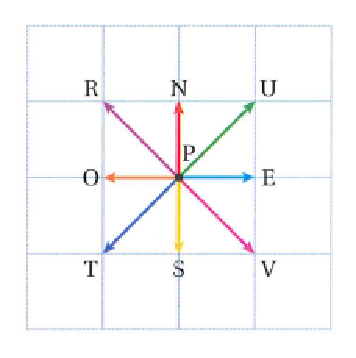
\includegraphics[scale=0.7]{exo-4-guitare.eps}$$
On donne le quadrillage ci-dessous et un point $A$.
$$\begin{pspicture}(20,8)
\psgrid[gridlabels=0,subgriddiv=0,griddots=10](20,8)   
\psdots(0,4)
\rput(0.2,4.2){$A$}
\end{pspicture}$$
\begin{enumerate}[$\diamond$]
\item 
		\begin{enumerate}[$a.$]
		\item Construire le point $B$, image du point $A$ par la translation de vecteur $\V{PN}$. 
		\item Construire le point $C$ tel que :
		$$\V{BC}=\V{PU}+\V{PN}$$ 
		\item Construire le point $D$ tel que $\V{CD}=2\V{PE}$.
		\item Construire le point $F$ tel que :
		$$\V{DF}=2\V{PS}+2\V{PE}$$
		\end{enumerate}
\item
		\begin{enumerate}[$a.$]
		\item Construire le point $G$, image du point $F$ par la translation de vecteur $\V{PE}$.
		\item Construire le point $H$ tel que :
		$$\V{GH}=\V{PH}+\V{HU}$$
		\item Construire le point $I$ tel que $\V{HI}=-\V{OP}$.
		\item Construire le point $J$ tel que :
		$$\V{IJ}=\V{PV}+0,5\V{PS}$$
		\item Construire le point $K$ tel que $\V{JK}=5\V{PE}$.
		\item Construire le point $L$ tel que :
		$$\V{KL}=0,5\V{PN}+\V{PE}$$
		\item Construire le point $M$ tel que :
		$$\V{LM}=3\V{PU}-3\V{PN}+\V{PO}$$
		\item Construire le point $Q$ tel que :
		$$\V{MQ}=\V{PT}-\V{PO}$$
		\end{enumerate}
\item Tracer la ligne bris�e $ABCDFGHIJKLMQ$.
\item Finir la construction par sym�trie de la ligne bris�e par rapport � la droite $(AQ)$. Quel objet reconnaissez-vous ?
\end{enumerate}





\end{document}
